\chapter{Parameter Estimation Process}
\label{ch: Estimation}

Parameter estimation problems can be interpreted as optimization problems, where one must find the optimal values of parameters in order to reduce error between real system and model when the same disturbance is applied to it. the error vector $e$ at any instant $t$ is calculated as the difference between the output vectors $y_{r}$, measured on the real system, and $y$, obtained from the model equations, as presented below.

\begin{equation}
	e(t) = y_{r}(t) - y(t)
	\label{eq: error_vector}
\end{equation}

The $l^{2}$-norm of error vector, denoted by $J$, is applied to evaluate how well the model describes the real system behaviour. The norm is obtained through equation \eqref{eq: J(p)}. It is important to notice that, since $y$ varies with $p$, so does $J$. The constant $\frac{1}{2}$ is only used for further simplification.

\begin{equation}
	J(p) = \frac{1}{2} \int\displaylimits_{0}^{T_{0}}\lVert e(t)\rVert_{2}dt = \frac{1}{2}\int\displaylimits_{0}^{T_{0}}e(t)^{T}\cdot e(t)dt
	\label{eq: J(p)}
\end{equation}

Many methods were developed for solving optimization problems, but two approaches have been largely employed during the last years. The first approach applies metaheuristics to obtain a sufficiently good solution. These methods are used in a variety of fields, ranging from biology to engineering, due to the fact that they are not developed for a specific type of problem.

Metaheuristics employ a stochastic search to find near-optimal solutions inside a given region. However, those methods often take a great amount of time to converge to a solution \cite{Blum2003}. Examples of metaheuristics are Ant Colony Optimization, Differential Evolution, Particle Swarm Optimization and Genetic Algorithm. Applications of this approach in electrical power system cases can be found in \cite{Todorovski2006} and \cite{Yoshida2000}.

The second approach applies analytical methods to find the local optimum solution from equations derived from the problem. Thus, they are problem specific and must be adapted from one case to another. Analytical methods often converge in few iterations, reducing processing time, but they are sensitive to initial conditions. Some examples of analytical methods are Newton's Method, Kalman Filter, Unscented Kalman Filter, etc.

By combining both approaches, the resulting method is expected to reduce the effects of their disadvantages and improving overall convergence. Mean-Variance Mapping Optimization (MVMO) was the metaheuristic chosen for this problem, alongside Trajectory Sensitivity Method (TSM) as analytical method. Both methods will be discussed in the following sections.

\section{Mean-Variance Mapping Optimization Method}

Presented in \cite{Erlich2010}, this metaheuristic based in evolution of populations shares characteristics with other evolutionary algorithms, but differ from them on how to induce mutations on the offspring in order to diversify the population. By considering statistical data of population during mutation process, MVMO introduces a memory factor to it, enhancing search mechanism. Due this factor, MVMO performs better than similar metaheuristics when population size is relatively small \cite{Nakawiro2011}. The terms `gene', `individuals' and `population' refer to `parameter', `parameter vector' and `set of parameter vectors' in MVMO, for the sake of analogy.

Two other relevant concepts largely used on metaheuristics are exploration and exploitation. The first one refers to a broad search carried through the region of interest. On the other hand, exploitation means the search on a small neighbourhood close to the best solutions.

Before starting the parameter search process, a few settings must be done, such as population size, number of offspring, number of genes selected for mutation and selection method. Also, the search region is defined by setting the range within genes can vary. This constrains the parameters values within a feasible region, preventing divergence. The search region is later normalized for all genes, aiding the estimation process. Termination criteria is also set in this step. In this work, both number of generations and error will be used as stop criteria.

After that, a randomly-distributed population is generated, evaluated and sorted. Moreover, the mean and variance of every gene in each population are calculated. These values will later be used on the mutation process. The individual with lower error is selected as parent for a new generated individual. The offspring is then created following three steps common in evolutionary algorithms: gene selection, mutation and crossover. After creation, the offspring is introduced to the population and the worst individual is discarded, as depicted in Figure \ref{fig: MVMOprocess}.

\begin{figure}[h]
	\caption{Exemplification of MVMO process}
	\begin{center}
		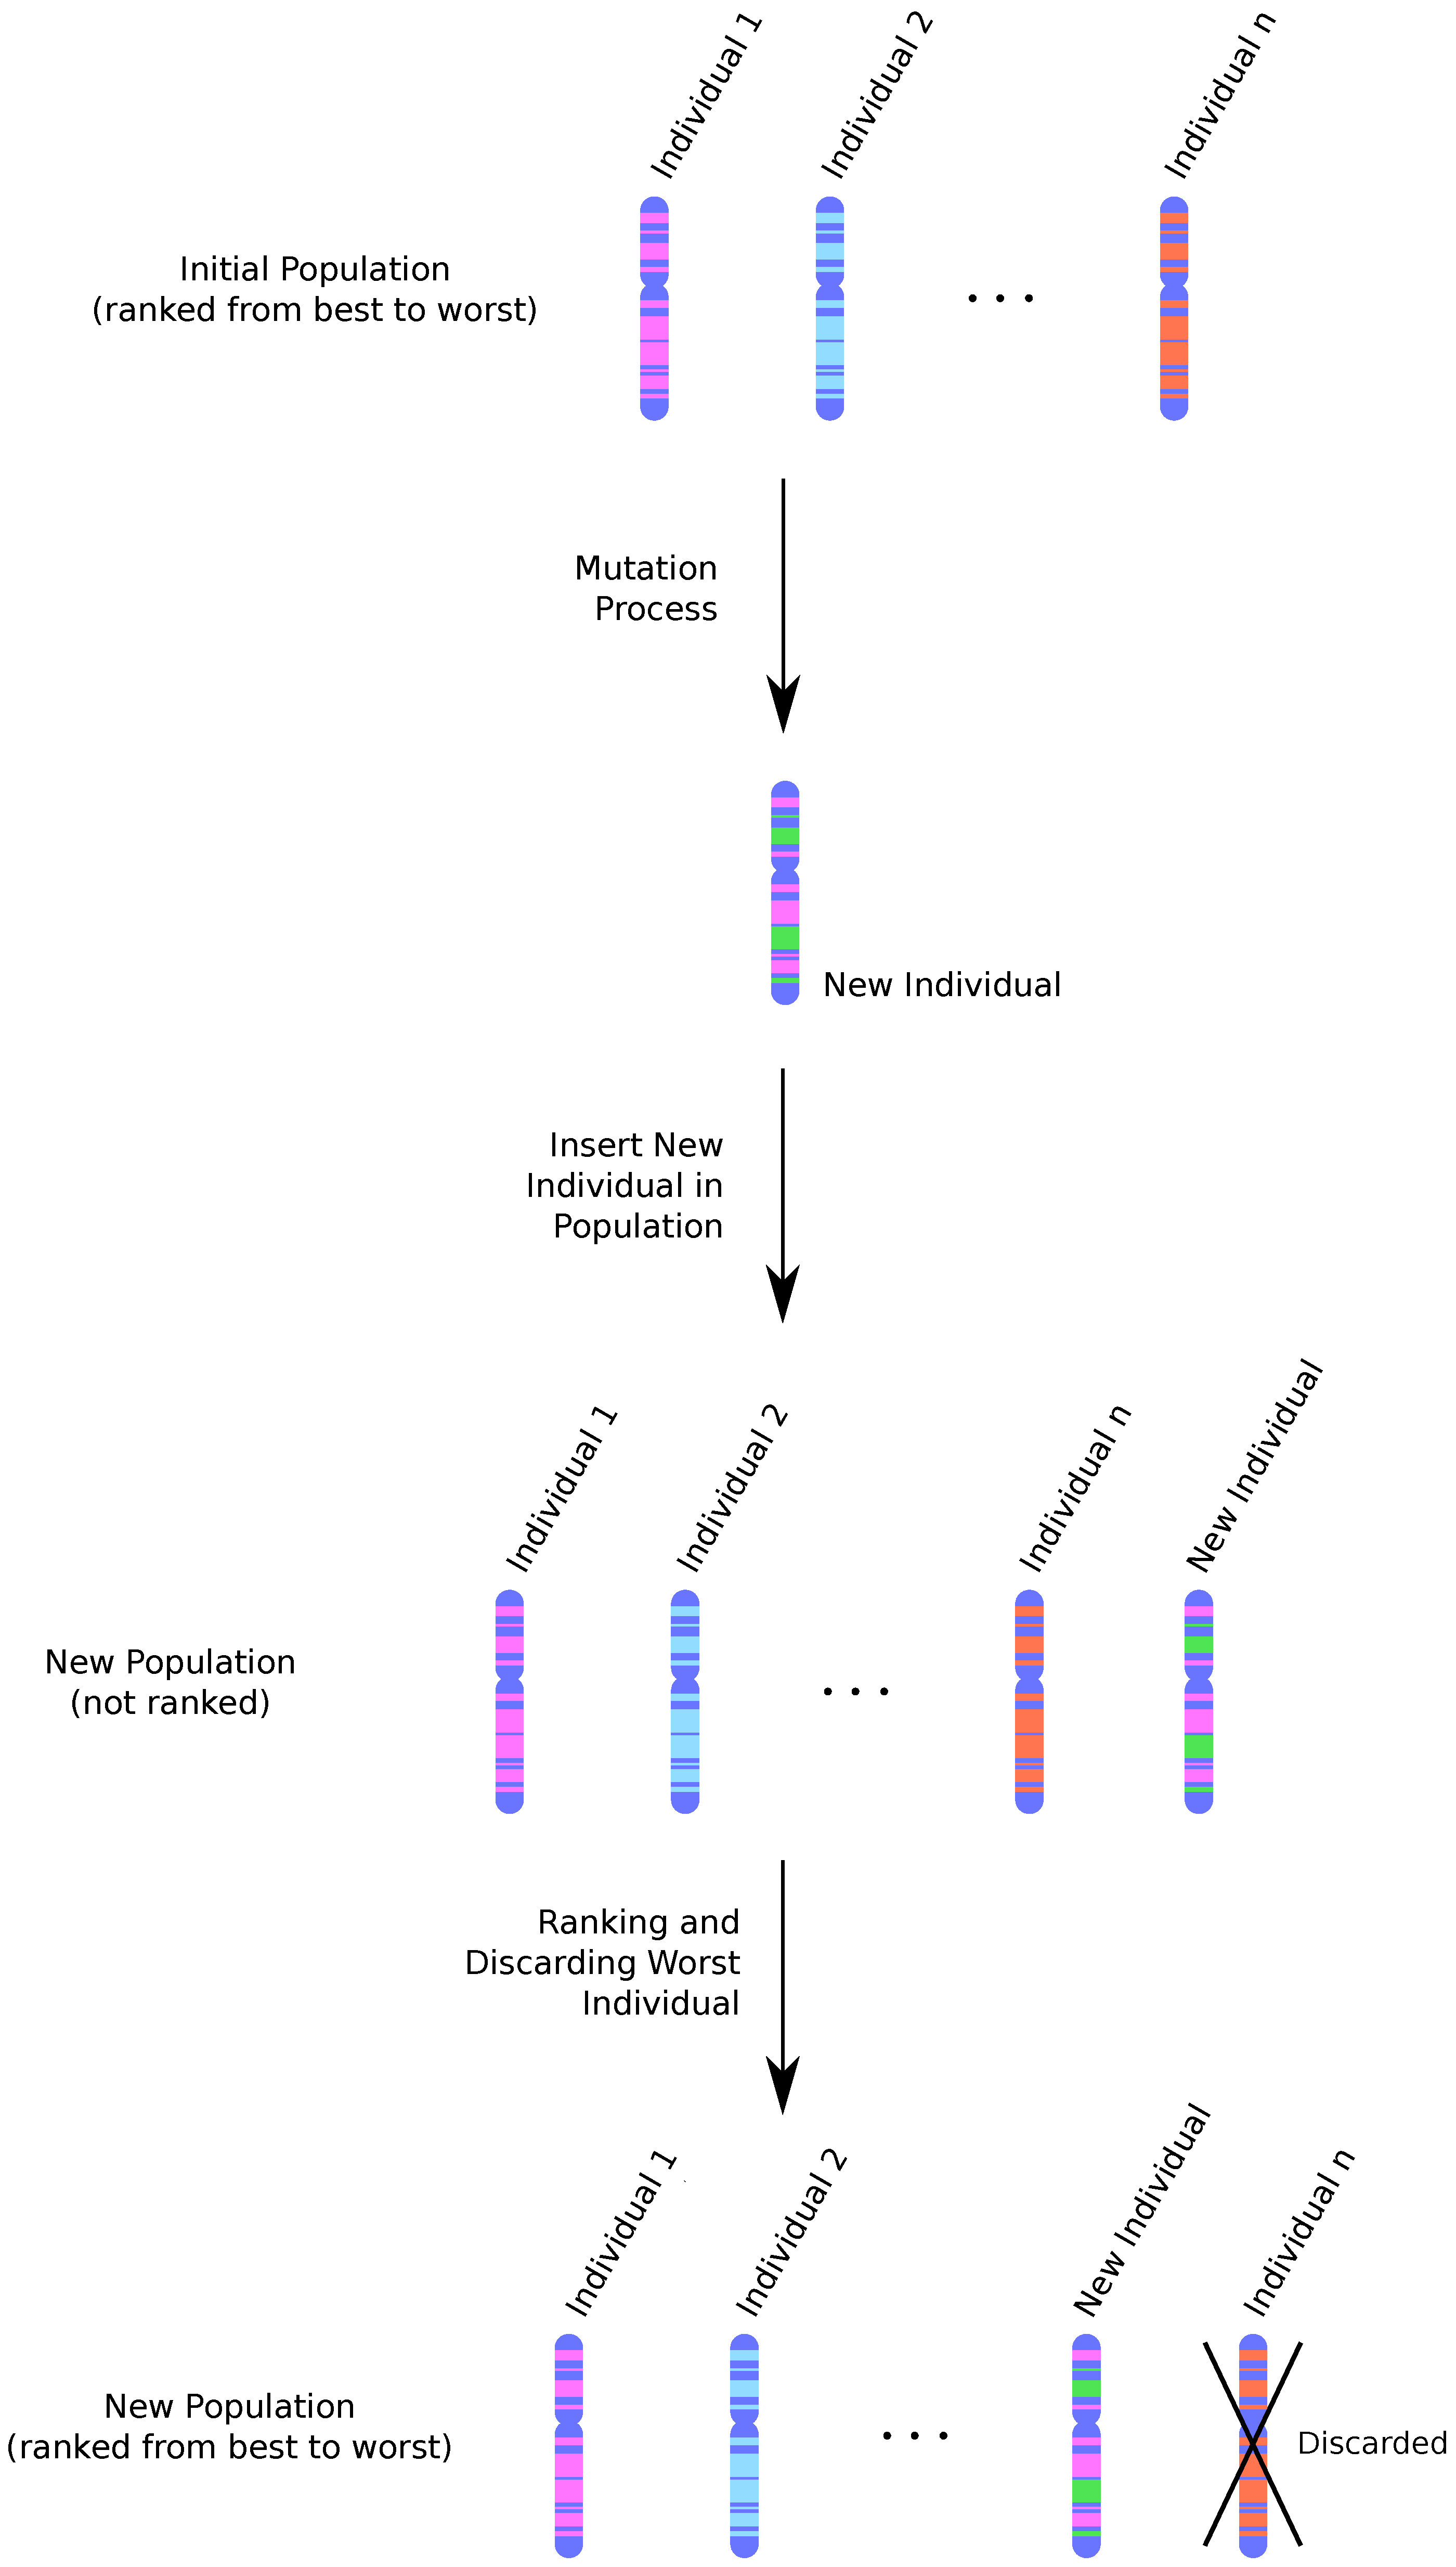
\includegraphics[scale=.2]{Images/MVMO_process2.eps}
	\end{center}
	\label{fig: MVMOprocess}
\end{figure}

\textbf{Gene selection} can be done in many ways and even vary throughout the estimation process, with strategies' efficiency depending on the problem. However, three strategies are commonly used in this step. The first one is comprised of randomly selecting which genes will suffer mutation and which will be directly inherited from the parent. Gene selection can also be done by a moving window approach or even a combination of both strategies, with part of the genes selected at random and other through the window.

\textbf{Mutation} step takes place after gene selection. At first, each selected gene receives a random value $\tilde{p}$ between [0,1] that will be used as an input to a mapping function based on the mean and variance of each particular gene on the population. Variance $v_{i}$ will directly influence on the shape factor $s_{i}$,  given by \eqref{eq: shapefac}, where $f_{s}$ is the scaling factor responsible for focusing on exploration or exploitation. In the event of zero variance, the last non-null value of $v_{i}$ is used.

\begin{equation}
	s_{i} = -f_{s}ln(v_{i})
	\label{eq: shapefac}
\end{equation}

Shape factor and mean value of genes of the population are used as inputs to a transformation function $h$, detailed in \eqref{eq: hfunc}. The final value of the gene is obtained through the mapping function described by equation \eqref{eq: mappingf}, where $h_{p} = h(u_{i} = \tilde{p})$, $h_{1} = h(u_{i} = 1)$ and $h_{0} = h(u_{i} = 0)$. It is important to notice that the mapping function will always provide a result in the interval [0,1], not violating the normalization made at beginning.

\begin{equation}
	h(\bar{p_{i}}, s_{i1}, s_{i2}, u_{i}) = \bar{p_{i}}(1 - e^{-u_{i}s_{i1}}) + (1 + \bar{p_{i}})e^{-(1 - u_{i})s_{i2}}
	\label{eq: hfunc}
\end{equation}

\begin{equation}
	p_{i} = h_{p} + (1 - h_{1} + h_{0})\tilde{p} - h_{0}
	\label{eq: mappingf}
\end{equation}

The resulting mapping function is depicted in Figure \ref{fig: mappingf}. The effects of different mean and shape factor values can be observed on Figure \ref{fig: mapeffects}.

\begin{figure}[!h]
	\caption{Example of MVMO mapping function}
	\begin{center}
		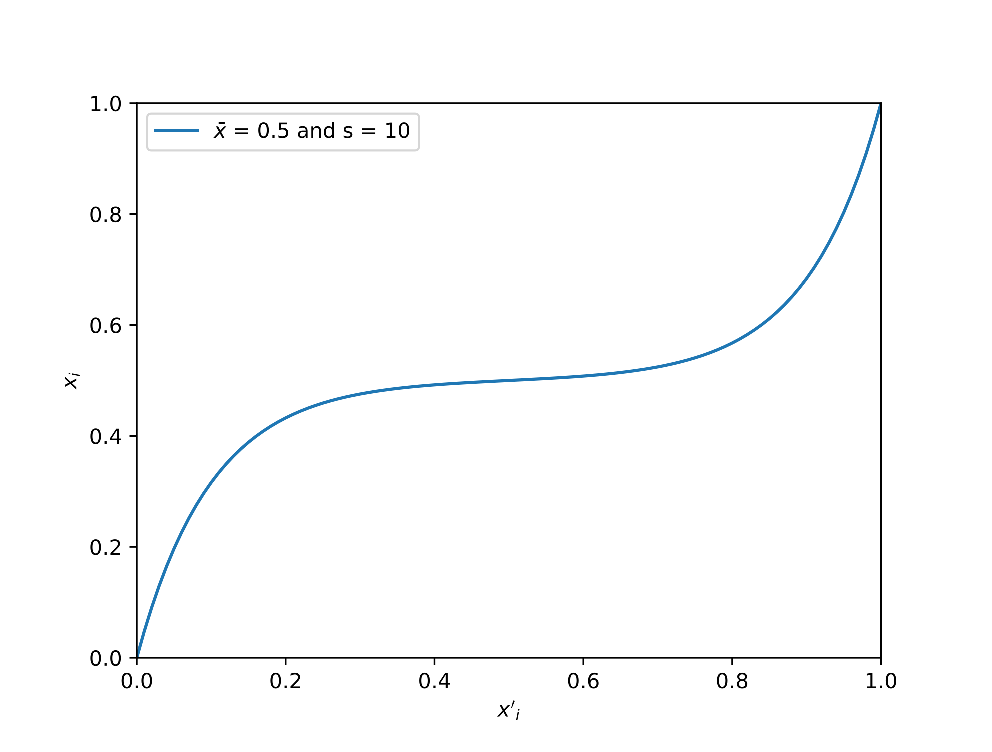
\includegraphics[scale=.5]{Images/MVMOTransformation.eps}
	\end{center}
	\label{fig: mappingf}
\end{figure}

\begin{figure}[h]
	\caption{Effect of different mean and shape factor values on mapping function}
	\begin{center}
		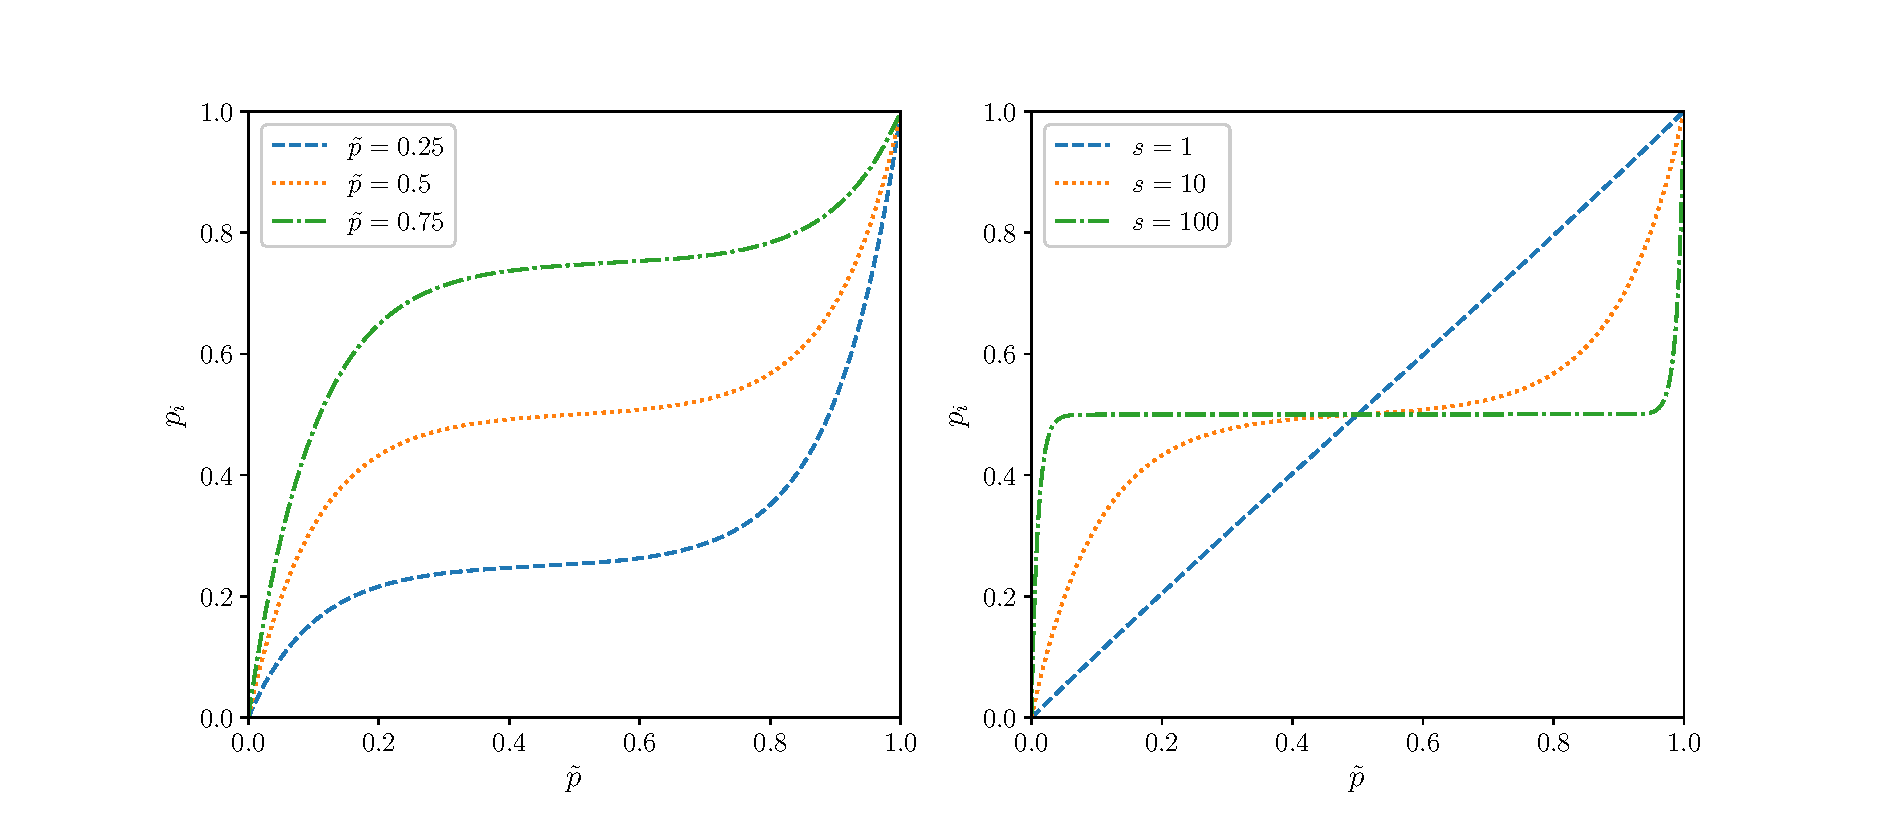
\includegraphics[scale=.5]{Images/mean_var_effects.eps}
	\end{center}
	\label{fig: mapeffects}
\end{figure}

As shown in \eqref{eq: hfunc}, two shape factors are used to evaluate the function. Different values of shape factors emphasizes the search below or above mean value. Thus, by controlling the values $s_{i1}$ and $s_{i2}$, the method can prioritize exploration (global search) or exploitation (local search) on a given region. Figure \ref{fig: diffs} depicts how asymmetrical shape factors affect the mapping function.

\begin{figure}[h]
	\caption{Comparison between symmetrical and asymmetrical shape factors}
	\begin{center}
		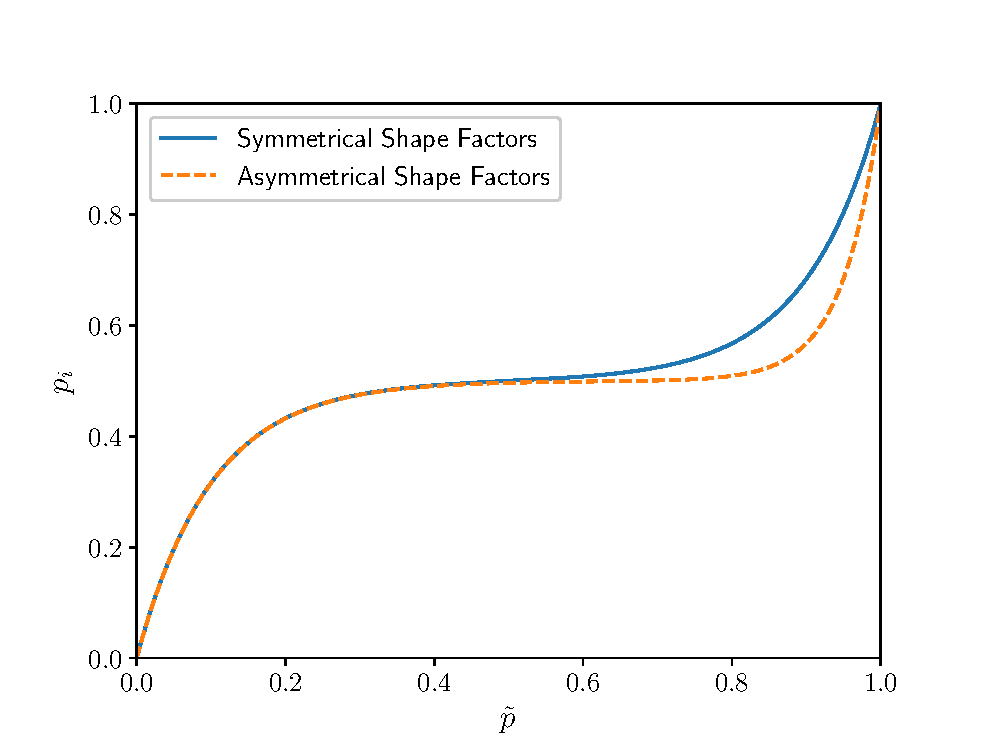
\includegraphics[scale=.5]{Images/symmetrical_transf.eps}
	\end{center}
	\label{fig: diffs}
\end{figure}

The final step during offspring generation is crossover. During this phase, the mutated genes are united with the remaining genes inherited from parent, forming the new individual. This new individual is evaluated and included to the population if it is better than, at least, the population's worst individual. This process goes on until at least one stop criterion has been fulfilled.

The main advantages of this method are low computational cost, good performance using small populations, constrained search region, preventing divergence, and the fact that it is non-specific. On the other hand, this method, as other metaheuristics, takes a great amount of time to converge when its error approaches zero.

\section{Trajectory Sensitivity Method}

Considering a nonlinear system described by \eqref{eq: xdot}, in order to minimize the error between model and real system, given by \eqref{eq: J(p)}, one must discover a parameter vector $p^{*}$ such as:

\begin{equation}
	G(p^{*}) = \frac{\partial J(p^{*})}{\partial p} = 0
\end{equation}

This derivative can be written as:

\begin{equation}	
	G(p) = -\int\displaylimits_{0}^{T_{0}} \left(\frac{dy}{dp}\right)^{T} (y_{r} - y) dt
	\label{eq: G(p)}
\end{equation}

Truncating the Taylor series for $G(p)$ on the first-order term results on \eqref{eq: Taylor}. The matrix $\Gamma$ is described in \eqref{eq: Gamma}.

\begin{equation}
	G(p^{*}) = G(p) + \Gamma (p)(p^{*} - p)
	\label{eq: Taylor}
\end{equation}

\begin{equation}
	\Gamma (p) = \frac{\partial G(p)}{\partial p} \approx \int\displaylimits_{0}^{T_{0}} \left(\frac{dy}{dp}\right)^{T} \left(\frac{dy}{dp}\right) dt
	\label{eq: Gamma}
\end{equation}

By rearranging the terms on \eqref{eq: Taylor}, the following equation is obtained. It describes how the parameters are updated after the $n^{th}$ iteration.

\begin{equation}
	p^{n+1} = p^{n} + \Gamma^{-1}(p^{n})\cdot G(p^{n})
\end{equation}

Obtaining the Jacobian matrix (also called trajectory sensitivity matrix) $\frac{\partial y}{\partial p}$, used in \eqref{eq: G(p)} and \eqref{eq: Gamma}, analytically is a hard task. However, by applying the definition of derivative, given by \eqref{eq: deriv}, the sensibilities can be approximated without any analytical derivation of the equations.

\begin{equation}
	\frac{df(x)}{dx} = \lim\limits_{\delta \to 0} \frac{f(x + \delta) - f(x)}{\delta}
	\label{eq: deriv}
\end{equation}

Consider two parameter vectors $p$ and $p^{\epsilon}$, where $p^{\epsilon}$ is obtained by adding a small perturbation $\epsilon p_{i}$ to the $i-th$ element of $p$, as shown in \eqref{eq: pvecs}.

\begin{equation}
	p = 
	\begin{bmatrix}
		p_{1} \\
		\vdots \\
		p_{i} \\
		\vdots \\
		p_{n}
	\end{bmatrix}; \ \ \ \ 
	 p^{\epsilon} =
	\begin{bmatrix}
		p_{1} \\
		\vdots \\
		p_{i} + \epsilon p_{i} \\
		\vdots \\
		p_{n}
	\end{bmatrix}
	\label{eq: pvecs}
\end{equation}

With $\epsilon$ sufficiently small, the partial derivative with respect to the parameter $p_{i}$ can be approximated by the difference shown in equation \eqref{eq: diff}. The value of $\epsilon = 0.1 \times 10^{-3}$ have shown great results for most cases. Using the approximation of the partial derivatives allows Trajectory Sensitivity method to be applied on both differentiable and non-differentiable systems \cite{Benchluch1993}, \cite{Cari2006}.

\begin{equation}
	\frac{\partial y(x, p, u)}{\partial p_{i}} \approx \frac{y(x, p^{\epsilon}, u) - y(x, p, u)}{\epsilon p_{i}}
	\label{eq: diff}
\end{equation}

The Trajectory Sensitivity Method has fast convergence characteristics and can applied directly to nonlinear problems, not requiring linearization. Also, by analyzing the sensitivities, the method provides information about identifiability of parameters. However, TSM is very sensitive to initial value of parameter chosen as starting point. Thus, if the initial values are too far from the real values, the method can either diverge or converge to wrong values. Besides, the information provided to the method must contain the effects of the parameters, otherwise they won't be observable \cite{Benchluch1993}.

\section{Hybrid Estimation Method}
\label{sec: Hybrid_Method}

By associating MVMO and TSM, the hybrid estimation approach applied in this work combines most benefits of both methods whilst mitigating their disadvantages. The resulting method has smaller convergence time when compared to MVMO alone and is less sensitive to initial values of parameters than TSM.

The flowchart depicted in Figure \ref{fig: flowchart} illustrates how this method works. At first, a disturbance occurs, resulting in a dynamic response of the real system. While $J(p)$ is greater than a given tolerance $tol_{1}$, MVMO algorithm will look for possible optimal solutions across the search region. Afterwards, the error will eventually drop to a value lower than $tol_{1}$, and TSM will be used to refine the search to an optimal solution, with error level below tolerance $tol_{2}$.

\begin{figure}[!h]
	\caption{Flowchart of estimation method}
	\begin{center}
		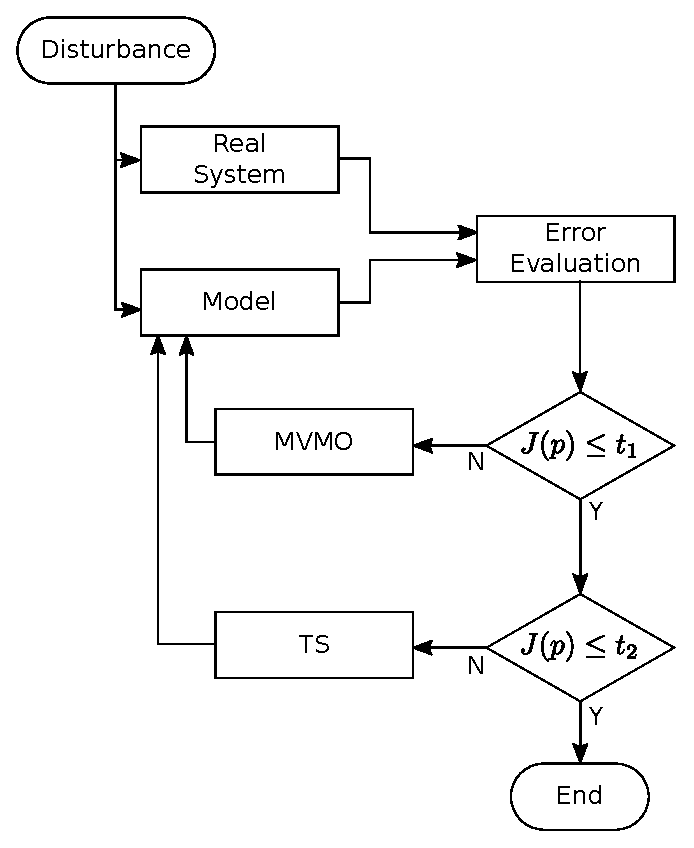
\includegraphics[scale=0.7]{Images/Flowchart.eps}
	\end{center}
	\label{fig: flowchart}
\end{figure}
